\documentclass[10pt,c,intlimits,aspectratio=1610]{beamer}
\usetheme{TUGSFB}
% the theme sets left=7mm but right=4mm -> make the side margins symmetric
\renewcommand{\indright}{\indleft}
\setbeamersize{text margin left=\indleft, text margin right=\indleft}

\usepackage[T1]{fontenc}
\usepackage[utf8]{inputenc}
\usepackage[english]{babel}
\usepackage[largesc]{newtxtext}
\renewcommand{\familydefault}{\sfdefault}
\usepackage[varg]{newtxmath}
\usepackage{amssymb,amsmath,mathtools}
\usepackage{booktabs}
\usepackage{siunitx}
\usepackage{tikz}
\usetikzlibrary{calc,arrows.meta,positioning,backgrounds,patterns,shapes.geometric}
\usepackage{pgfplots}
\pgfplotsset{compat=1.18}
\pgfplotsset{every axis/.append style={thick}}
\usepgfplotslibrary{colormaps}

\graphicspath{{./}{data/}}

% ---- colours / shortcuts -----------------------------------------------------
\definecolor{dpBlue}{RGB}{0,103,173}   % Mech_blau
\definecolor{dpRed}{RGB}{247,1,70}     % TUG_rot
\newcommand{\R}{\mathbb{R}}
\newcommand{\Om}{\Omega}
\newcommand{\dd}{\,\mathrm{d}}
\newcommand{\Gs}{\Gamma_{\mathrm s}}
\newcommand{\highlight}[1]{{\color{dpRed}#1}}

% ---- title metadata ----------------------------------------------------------
\title[Optimal placement of plate stiffeners]%
{Optimal Placement of Plate Stiffeners\\[1mm]
 \large A FreeFEM Shape-Optimization Study}
\author[K.\,Brkovic, L.\,M.\,Han]{Katharina Brkovic \and Luis Mathias Han}
\institute{Optimization Methods for Sustainable Building Constructions}
\date{June 2026}

\begin{document}

% =============================================================================
\mytitle
\addtocounter{framenumber}{-1}

% -----------------------------------------------------------------------------
\begin{frame}{Outline}
  \tableofcontents
\end{frame}

% #############################################################################
\section{Problem statement}
% #############################################################################

% ---- motivation -------------------------------------------------------------
\begin{frame}{Why stiffen a plate?}
  \begin{columns}[c]
    \begin{column}{0.54\textwidth}
      \begin{itemize}
        \item A thin plate carries transverse load mainly by \highlight{bending}
              and is therefore very compliant.
        \item Welding slender \highlight{stiffeners} (ribs) onto it raises the
              stiffness drastically at almost no added weight.
        \item The \highlight{position} of the stiffeners decides how much they
              help $\;\Rightarrow\;$ a \highlight{shape-optimization} problem.
      \end{itemize}
      \vspace{2mm}
      \textbf{Goal:} place the stiffeners so that the loaded plate deflects as
      little as possible.
    \end{column}
    \begin{column}{0.46\textwidth}
      \centering
      % section through the slab: thin plate on top, deep down-stand ribs below
      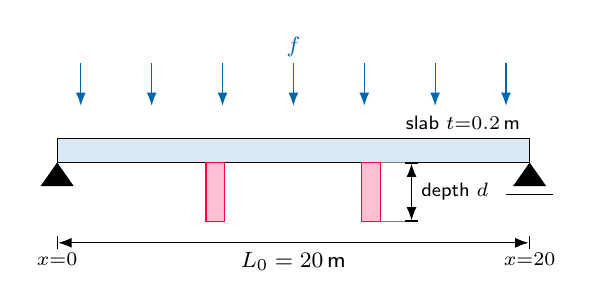
\begin{tikzpicture}[scale=0.3,>=Latex]
        % load
        \foreach \x in {1,4,7,10,13,16,19}{\draw[->,dpBlue] (\x,4.2)--(\x,2.4);}
        \node[dpBlue] at (10,4.9){\footnotesize $f$};
        % slab (thin, t = 0.2 m)
        \fill[dpBlue!15] (0,0) rectangle (20,1); \draw (0,0) rectangle (20,1);
        \node[above left] at (20,1){\scriptsize slab $t{=}0.2$\,m};
        % down-stand ribs (depth d)
        \foreach \x in {6.7,13.3}{
          \fill[dpRed!25] (\x-0.4,0) rectangle (\x+0.4,-2.5);
          \draw[dpRed]    (\x-0.4,0) rectangle (\x+0.4,-2.5);}
        % simple supports (pin / roller)
        \fill (0,0)--(-0.7,-1)--(0.7,-1)--cycle;
        \fill (20,0)--(19.3,-1)--(20.7,-1)--cycle; \draw (19.0,-1.35)--(21.0,-1.35);
        % dimensions
        \draw[|<->|] (0,-3.4)--(20,-3.4) node[midway,below]{\footnotesize $L_0=20$\,m};
        \node[below] at (0,-3.4){\scriptsize $x{=}0$};
        \node[below] at (20,-3.4){\scriptsize $x{=}20$};
        \draw[gray,thin] (13.7,0)--(15.0,0);
        \draw[gray,thin] (13.7,-2.5)--(15.0,-2.5);
        \draw[|<->|] (15.0,0)--(15.0,-2.5) node[midway,right]{\scriptsize depth $d$};
      \end{tikzpicture}\\[0.5mm]
      {\scriptsize\itshape section: thin slab + \textcolor{dpRed}{down-stand ribs}
        (vert.\ exaggerated)}
    \end{column}
  \end{columns}
\end{frame}

% ---- mechanical model -------------------------------------------------------
\begin{frame}{Mechanical model}
  \begin{columns}[t]
    \begin{column}{0.5\textwidth}
      \textbf{Plate} (Kirchhoff thin plate)
      \begin{itemize}
        \item deflection field $w(x,y)$ on $\Om=(0,L_0)\times(0,H_0)$
        \item bending stiffness $D=\dfrac{E\,t^3}{12(1-\nu^2)}$,\; Poisson ratio $\nu$
      \end{itemize}
      \vspace{1mm}
      \textbf{Stiffeners} (beams on lines $\Gs$)
      \begin{itemize}
        \item smeared onto interior lines -- \highlight{no extra DOFs}
        \item add bending stiffness $EI$ and torsional stiffness $GI_t$
              \emph{along} the line
      \end{itemize}
    \end{column}
    \begin{column}{0.5\textwidth}
      \textbf{Load \& assumptions}
      \begin{itemize}
        \item uniform transverse pressure $f$
        \item stiffener axis in the plate mid-surface
              ($\Rightarrow$ no bending--membrane coupling, a deliberate
              simplification)
        \item small deflections (linear theory)
      \end{itemize}
      \vspace{1mm}
      \centering
      % zoomed section: thin plate (D, nu) + one down-stand rib (EI, GIt)
      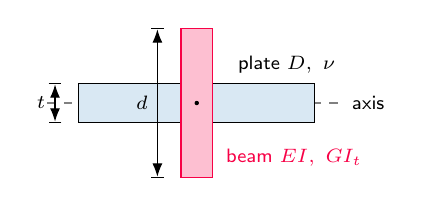
\begin{tikzpicture}[scale=0.5,>=Latex]
        % common centroidal axis = plate mid-surface
        \draw[dashed,gray] (-0.8,0)--(6.7,0) node[right,black]{\scriptsize axis};
        % plate: thin strip centred on the mid-surface
        \fill[dpBlue!15] (0,-0.5) rectangle (6,0.5); \draw (0,-0.5) rectangle (6,0.5);
        \node[above right] at (3.8,0.5){\scriptsize plate $D,\ \nu$};
        % beam: depth d, centroid on the SAME axis -> no eccentricity
        \fill[dpRed!25] (2.6,-1.9) rectangle (3.4,1.9); \draw[dpRed] (2.6,-1.9) rectangle (3.4,1.9);
        \node[dpRed,right] at (3.5,-1.4){\scriptsize beam $EI,\ GI_t$};
        % coincident centroids on the axis
        \fill (3.0,0) circle (1.6pt);
        \draw[|<->|] (-0.6,-0.5)--(-0.6,0.5) node[midway,left]{\scriptsize $t$};
        \draw[|<->|] (2.0,-1.9)--(2.0,1.9) node[midway,left]{\scriptsize $d$};
      \end{tikzpicture}\\[0.5mm]
      {\scriptsize\itshape beam centroid in the plate mid-surface
        $\Rightarrow$ no eccentricity}
    \end{column}
  \end{columns}
\end{frame}

% ---- governing equations ----------------------------------------------------
\begin{frame}{Governing equations (strong form)}
  \textbf{Plate} -- 4\textsuperscript{th}-order Kirchhoff equation
  \begin{equation*}
     D\,\Delta^2 w \;=\; f \qquad \text{in } \Om,
     \qquad \Delta^2 = \partial_{xxxx}+2\,\partial_{xxyy}+\partial_{yyyy}.
  \end{equation*}
  \textbf{Stiffener} on a line $\Gs$ with tangent $\boldsymbol t$ -- an
  Euler--Bernoulli beam in the deflection $w|_{\Gs}$:
  \begin{equation*}
     EI\,\partial_{ssss}w \quad\text{(bending)} \qquad
     GI_t\,\partial_{ss}\theta \quad\text{(torsion)},\qquad
     s = \text{arc length along } \boldsymbol t .
  \end{equation*}
  \vspace{1mm}
  \textbf{Boundary conditions} (two per edge, because the PDE is
  4\textsuperscript{th} order):
  \begin{center}
  \emph{clamped} \;($w=0,\ \partial_n w =0$)\quad$\bullet$\quad
  \emph{simply supported} \;($w=0,\ M_n=0$)\quad$\bullet$\quad
  \emph{free} \;($M_n=0,\ V_n=0$).
  \end{center}
\end{frame}

% ---- optimization problem ---------------------------------------------------
\begin{frame}{Optimization problem}
  \textbf{Design variables:} stiffener positions
  $\boldsymbol s = (s_1,\dots,s_{n})$ (the interior dividing lines).

  \medskip
  \textbf{Objective: compliance} = work done by the external load
  \begin{equation*}
     C(\boldsymbol s) \;=\; \int_\Om f\, w(\boldsymbol s)\,\dd\Om
     \;\longrightarrow\; \min .
  \end{equation*}
  Minimal compliance $\;\Leftrightarrow\;$ minimal stored energy
  $\;\Leftrightarrow\;$ \highlight{stiffest plate}.

  \medskip
  \textbf{Constraints} -- stiffeners stay ordered inside the plate
  (outer edges fixed):
  \begin{equation*}
     0 < s_1 < s_2 < \dots < s_n < L_0
     \qquad(\text{box constraints}).
  \end{equation*}
\end{frame}

% #############################################################################
\section{Weak form, boundary conditions and code}
% #############################################################################

% ---- weak form --------------------------------------------------------------
\begin{frame}{Weak form}
  Multiply by a test function $\delta w$ and integrate by parts twice:
  $a(w,\delta w)=\ell(\delta w)$ with
  \medskip

  \textbf{Plate bending energy} (full Kirchhoff form with Poisson coupling):
  \begin{equation*}
    a_{\text{plate}}=\!\int_\Om \! D\Big[
      w_{xx}\delta w_{xx}+w_{yy}\delta w_{yy}
      +\nu\,(w_{xx}\delta w_{yy}+w_{yy}\delta w_{xx})
      +2(1-\nu)\,w_{xy}\delta w_{xy}\Big]\dd\Om
  \end{equation*}

  \textbf{Stiffener bending + torsion} on the lines $\Gs$
  ($\boldsymbol n$ = line normal):
  \begin{align*}
    a_{\text{beam}}&=\int_{\Gs} EI\;\kappa_{ss}(w)\,\kappa_{ss}(\delta w)\dd s,
       &\kappa_{ss}&= w_{xx}n_y^2-2w_{xy}n_xn_y+w_{yy}n_x^2,\\[1mm]
    a_{\text{tor}}&=\int_{\Gs} GI_t\;\kappa_{sn}(w)\,\kappa_{sn}(\delta w)\dd s,
       &\kappa_{sn}&= n_xn_y(w_{yy}-w_{xx})+(n_x^2-n_y^2)\,w_{xy}.
  \end{align*}

  \textbf{Load:}\; $\ell(\delta w)=\int_\Om f\,\delta w\dd\Om$.
  \hfill{\footnotesize\highlight{$a_{\text{plate}}$ ($\nu$) and $a_{\text{tor}}$ are our additions to the base code.}}
\end{frame}

% ---- how the forms were obtained --------------------------------------------
\begin{frame}{How the gradients were obtained}
  \begin{columns}[c]
    \begin{column}{0.6\textwidth}
      \begin{itemize}
        \item The weak form (energy) is written by hand; the
              \highlight{shape gradients} -- the derivatives of the
              compliance w.r.t.\ the stiffener positions -- are derived
              \highlight{symbolically} with \texttt{autofreefem} (SymPy):
              \begin{itemize}
                \item define the Lagrangian (energy $-$ load),
                \item let it compute the \highlight{shape derivative}
                      of the compliance,
                \item auto-translate the gradient to FreeFEM syntax.
              \end{itemize}
        \item This removes hand-algebra errors in the lengthy
              $\nu$- and torsion-terms.
        \item Script: \texttt{autofreefem/run\_plateStiffener.py}.
      \end{itemize}
    \end{column}
    \begin{column}{0.4\textwidth}
      \centering
      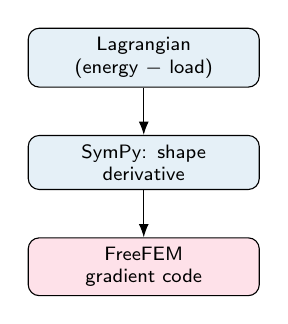
\begin{tikzpicture}[node distance=6mm,>=Latex,
          every node/.style={font=\scriptsize}]
        \node[draw,rounded corners,fill=dpBlue!10,text width=2.7cm,align=center](L){Lagrangian\\ (energy $-$ load)};
        \node[draw,rounded corners,below=of L,fill=dpBlue!10,text width=2.7cm,align=center](S){SymPy: shape\\ derivative};
        \node[draw,rounded corners,below=of S,fill=dpRed!12,text width=2.7cm,align=center](F){FreeFEM\\ gradient code};
        \draw[->] (L)--(S); \draw[->] (S)--(F);
      \end{tikzpicture}
    \end{column}
  \end{columns}
\end{frame}

% ---- boundary conditions ----------------------------------------------------
\begin{frame}{Boundary conditions -- three support types per edge}
  Each of the four edges can be set independently. A 4\textsuperscript{th}-order
  problem needs \highlight{two} conditions per edge:
  \medskip
  \begin{center}
  \renewcommand{\arraystretch}{1.35}
  \begin{tabular}{@{}lll@{}}
    \toprule
    \textbf{Support} & \textbf{Conditions} & \textbf{Numerical treatment}\\
    \midrule
    Clamped          & $w=0,\;\partial_n w=0$ & strong, \texttt{on(\,$\cdot$\,)} (set $w,w_x,w_y$)\\
    Simply supp.\ (hinged) & $w=0,\;M_n=0$ & penalty spring $\int_e c\,w\,\delta w$, \;rotation free\\
    Free             & $M_n=0,\;V_n=0$ & nothing added (\highlight{natural} BC)\\
    \bottomrule
  \end{tabular}
  \end{center}
  \vspace{2mm}
  \begin{itemize}
    \item Hinged: large spring stiffness $c=10^{15}$ pins $w\!\approx\!0$ while
          leaving the rotation free.
    \item \highlight{At least one edge must be supported} -- otherwise rigid-body
          modes make the system singular (the code asserts this).
  \end{itemize}
\end{frame}

% ---- code structure ---------------------------------------------------------
\begin{frame}{Code structure (FreeFEM)}
  \centering
  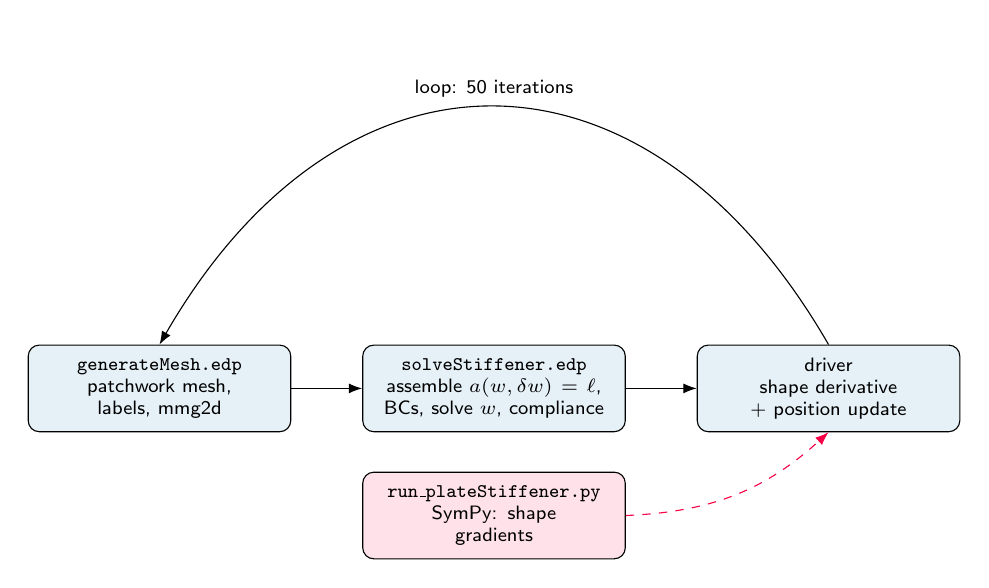
\begin{tikzpicture}[node distance=5mm and 9mm,>=Latex,
      box/.style={draw,rounded corners,fill=dpBlue!10,text width=3.1cm,
                  align=center,font=\scriptsize,minimum height=1.1cm}]
    \node[box](mesh){\texttt{generateMesh.edp}\\ patchwork mesh,\\ labels, mmg2d};
    \node[box,right=of mesh](solve){\texttt{solveStiffener.edp}\\ assemble $a(w,\delta w)=\ell$,\\ BCs, solve $w$, compliance};
    \node[box,right=of solve](deriv){driver\\ shape derivative\\ + position update};
    \node[box,below=of solve,fill=dpRed!12](py){\texttt{run\_plateStiffener.py}\\ SymPy: shape\\ gradients};
    \draw[->](mesh)--(solve); \draw[->](solve)--(deriv);
    \draw[->,dpRed,dashed](py.east)to[bend right=20](deriv.south);
    \draw[->](deriv.north)to[out=120,in=60,looseness=1.4]
        node[above,font=\scriptsize]{loop: 50 iterations}(mesh.north);
  \end{tikzpicture}
  \vspace{2mm}
  \begin{itemize}\footnotesize
    \item Each iteration: re-mesh $\to$ solve $\to$ gradient $\to$ move stiffeners;
          objective and deflection field are logged.
  \end{itemize}
\end{frame}

% #############################################################################
\section{Results}
% #############################################################################
% --- results frames are inserted here once the case matrix has finished ---
% =============================================================================
%  Results frames -- REAL UNITS (concrete slab).  Data: ./data (copy_data.sh)
%  Compliance C in kJ, deflection w in mm.
%  Uniform layout: big figure (left) + Setup / Findings (right).
% =============================================================================

% compact top-view deflection map: #1=width #2=file #3=title #4=meta max [mm]
\newcommand{\cmap}[4]{%
  \begin{tikzpicture}
    \begin{axis}[title={#3},width=#1,view={0}{90},axis equal image,
        enlargelimits=false,axis line style={draw=none},xtick=\empty,ytick=\empty,
        point meta min=0,point meta max=#4,colormap/viridis,
        title style={font=\scriptsize,yshift=-1.5mm}]
      \addplot3[surf,shader=interp,mesh/ordering=x varies] table {#2};
    \end{axis}
  \end{tikzpicture}}

% -----------------------------------------------------------------------------
\begin{frame}{Parametric study: a real reinforced-concrete slab}
  \begin{columns}[t]
    \begin{column}{0.54\textwidth}
      \textbf{Slab \& material}
      \begin{itemize}\small
        \item $20\times10$\,m, thickness $h=0.2$\,m
        \item concrete $E\approx33$\,GPa, $\nu=0.2$
        \item $D=\dfrac{E h^3}{12(1-\nu^2)}\approx \highlight{23}$\,MN\,m
        \item load $g{+}q\approx10$\,kN/m$^2$ $\Rightarrow f=0.01$\,MN/m$^2$
      \end{itemize}
    \end{column}
    \begin{column}{0.46\textwidth}
      \textbf{Stiffeners} (down-stand beams)
      \begin{itemize}\small
        \item $30\times50$\,cm: $EI\approx \highlight{103}$\,MN\,m$^2$
        \item $30\times100$\,cm: $EI\approx \highlight{825}$\,MN\,m$^2$ \;($8\times$)
        \item torsion $GI_t = 0.1\,EI$ (cracked, representative)
      \end{itemize}
      \vspace{1mm}
      \textbf{Conventions}
      \begin{itemize}\small
        \item supports: simply supported (base) \& clamped
        \item $C$ in kJ, $w$ in mm
        \item rib position $x$ measured from the left edge ($x{=}0$)
              along the $20$\,m span, $x\in(0,20)$\,m
      \end{itemize}
    \end{column}
  \end{columns}
  \vspace{1mm}
  {\footnotesize Realistically $EI/D\approx 4$--$36$, so rib \emph{placement} is a
  fine adjustment while \highlight{section} and \highlight{support} dominate.}
\end{frame}

% --- reference: convergence --------------------------------------------------
\begin{frame}{Reference case -- convergence}
  \begin{columns}[c]
    \begin{column}{0.58\textwidth}
      \centering
      \begin{tikzpicture}
        \begin{axis}[width=7.2cm,height=5.2cm,
            xlabel={iteration},ylabel={compliance $C$ [kJ]},
            xmin=0,xmax=80,ymin=26.4,ymax=29,
            tick label style={font=\scriptsize},label style={font=\small},
            grid=major,grid style={gray!20}]
          \addplot[dpBlue,very thick] table[col sep=comma,skip first n=1,
              x index=0,y index=1]{data/ref_obj.txt};
        \end{axis}
      \end{tikzpicture}
    \end{column}
    \begin{column}{0.42\textwidth}
      \textbf{Setup}
      \begin{itemize}\footnotesize
        \item simply supported, $30\times50$, $n_V=2$
        \item off-centred start $x=4,\,9$\,m
      \end{itemize}
      \textbf{Findings}
      \begin{itemize}\footnotesize
        \item ribs migrate to $x=\highlight{8.5,\,11.5}$\,m
        \item $C:\ 28.8\to\highlight{26.7}$\,kJ \;($-7.5\%$)
        \item smooth, monotone descent
      \end{itemize}
    \end{column}
  \end{columns}
\end{frame}

% --- reference: deflection before / after ------------------------------------
\begin{frame}{Reference case -- deflection before / after}
  \begin{columns}[c]
    \begin{column}{0.6\textwidth}
      \centering
      \cmap{6.0cm}{data/ref_w_init.dat}{start $x=4,9$ \;($w_{\max}=33.2$\,mm)}{34}\\[1mm]
      \cmap{6.0cm}{data/ref_w_final.dat}{optimized $x=8.5,11.5$ \;($w_{\max}=27.5$\,mm)}{34}\\[0.5mm]
      {\tiny colour: deflection $0\dots34$\,mm (viridis), slab to scale}
    \end{column}
    \begin{column}{0.4\textwidth}
      \textbf{Setup}
      \begin{itemize}\footnotesize
        \item simply supported, $30\times50$, $n_V=2$
      \end{itemize}
      \textbf{Findings}
      \begin{itemize}\footnotesize
        \item ribs cluster toward mid-span, where a simply supported slab
              deflects most
        \item peak deflection $33.2\to\highlight{27.5}$\,mm \;($-17\%$)
      \end{itemize}
    \end{column}
  \end{columns}
\end{frame}

% --- boundary conditions -----------------------------------------------------
\begin{frame}{Effect of the boundary conditions}
  \begin{columns}[c]
    \begin{column}{0.56\textwidth}
      \centering
      \cmap{4.0cm}{data/bcClamped_w_final.dat}{clamped \;($C=5.0$, $w_{\max}=6.3$)}{28}\\[0.5mm]
      \cmap{4.0cm}{data/bcOneway_w_final.dat}{one-way \;($C=8.9$, $w_{\max}=10.6$)}{28}\\[0.5mm]
      \cmap{4.0cm}{data/bcHinged_w_final.dat}{simply supp. \;($C=26.7$, $w_{\max}=27.5$)}{28}\\[0.5mm]
      {\tiny colour: deflection $0\dots28$\,mm}
    \end{column}
    \begin{column}{0.44\textwidth}
      \textbf{Setup}
      \begin{itemize}\footnotesize
        \item same slab, $30\times50$, $n_V=2$
        \item three support types
      \end{itemize}
      \textbf{Findings}
      \begin{itemize}\footnotesize
        \item support \highlight{dominates}: simply supported $\sim5\times$
              more compliant than clamped
        \item optimal rib positions $x$\,[m] are support-dependent
              (even start $6.7/13.3$):
              \begin{itemize}\footnotesize
                \item clamped $\to \highlight{7.6/12.4}$
                \item one-way $\to \highlight{5.0/15.0}$ \emph{(spread)}
                \item simply supp.\ $\to \highlight{8.5/11.5}$ \emph{(clustered)}
              \end{itemize}
      \end{itemize}
    \end{column}
  \end{columns}
\end{frame}

% --- number of stiffeners ----------------------------------------------------
\begin{frame}{Effect of the number of stiffeners}
  \begin{columns}[c]
    \begin{column}{0.56\textwidth}
      \centering
      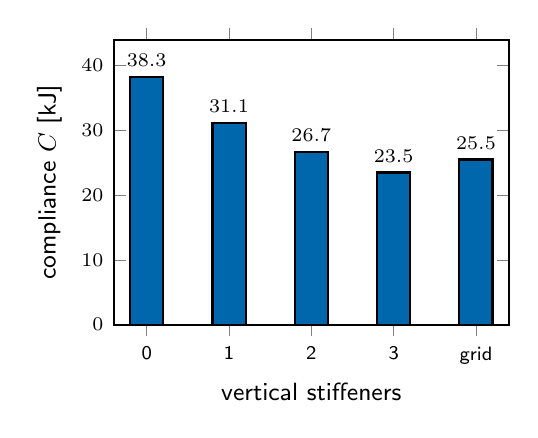
\begin{tikzpicture}
        \begin{axis}[ybar,width=6.6cm,height=5.2cm,
            ylabel={compliance $C$ [kJ]},xlabel={vertical stiffeners},
            symbolic x coords={0,1,2,3,grid},xtick=data,
            nodes near coords,nodes near coords style={font=\scriptsize},
            ymin=0,ymax=44,bar width=12pt,
            tick label style={font=\scriptsize},label style={font=\small}]
          \addplot[fill=dpBlue] coordinates
            {(0,38.3)(1,31.1)(2,26.7)(3,23.5)(grid,25.5)};
        \end{axis}
      \end{tikzpicture}\\[-0.5mm]
      {\tiny ``grid'' $=2$ vertical $+\,1$ horizontal stiffener}
    \end{column}
    \begin{column}{0.44\textwidth}
      \textbf{Setup}
      \begin{itemize}\footnotesize
        \item simply supported slab, $30\times50$ ribs
      \end{itemize}
      \textbf{Findings}
      \begin{itemize}\footnotesize
        \item each rib helps with \highlight{diminishing return}
              ($38\to23$\,kJ for $0\to3$)
        \item $3$ \emph{parallel} ribs beat the $2{+}1$ grid: the slab spans
              the short side, so ribs across it carry more
      \end{itemize}
    \end{column}
  \end{columns}
\end{frame}

% --- cross-section -----------------------------------------------------------
\begin{frame}{Effect of the stiffener cross-section}
  \begin{columns}[c]
    \begin{column}{0.6\textwidth}
      \centering
      \cmap{6.0cm}{data/bcHinged_w_final.dat}{$30\times50$\,cm \;($C=26.7$, $w_{\max}=27.5$)}{28}\\[1mm]
      \cmap{6.0cm}{data/cs825_w_final.dat}{$30\times100$\,cm \;($C=10.3$, $w_{\max}=10.0$)}{28}\\[0.5mm]
      {\tiny colour: deflection $0\dots28$\,mm}
    \end{column}
    \begin{column}{0.4\textwidth}
      \textbf{Setup}
      \begin{itemize}\footnotesize
        \item simply supported, $n_V=2$
      \end{itemize}
      \textbf{Findings}
      \begin{itemize}\footnotesize
        \item doubling the depth raises $EI$ \highlight{$8\times$} ($103\to825$)
        \item compliance \highlight{more than halves} ($26.7\to10.3$\,kJ)
        \item optimum shifts toward even-thirds, $x$\,[m]:
              \begin{itemize}\footnotesize
                \item $30\times50 \to \highlight{8.5/11.5}$ (clustered)
                \item $30\times100 \to \highlight{6.9/13.1}$ ($\approx 6.7/13.3$)
              \end{itemize}
      \end{itemize}
    \end{column}
  \end{columns}
\end{frame}

% --- torsion -----------------------------------------------------------------
\begin{frame}{Effect of stiffener torsion}
  \begin{columns}[c]
    \begin{column}{0.54\textwidth}
      \centering
      \renewcommand{\arraystretch}{1.3}
      \begin{tabular}{@{}lccc@{}}
        \toprule
        $30\times100$ rib & $GI_t$ & $C$ [kJ] & $w_{\max}$ [mm]\\
        \midrule
        with torsion    & $82.5$ & $10.3202$ & $10.00$\\
        without torsion & $0$    & $10.3202$ & $10.00$\\
        \midrule
        difference      & --     & $<0.01\%$ & $<0.01\%$\\
        \bottomrule
      \end{tabular}
    \end{column}
    \begin{column}{0.46\textwidth}
      \textbf{Setup}
      \begin{itemize}\footnotesize
        \item $30\times100$, simply supported, $n_V=2$
      \end{itemize}
      \textbf{Findings}
      \begin{itemize}\footnotesize
        \item torsion changes compliance by \highlight{$<0.1\%$} --
              negligible here
        \item it engages only where the plate \emph{twists} along the rib
              (asymmetric load, skew, corners)
        \item including it keeps the model general
      \end{itemize}
    \end{column}
  \end{columns}
\end{frame}

% --- discussion --------------------------------------------------------------
\begin{frame}{Discussion}
  \begin{itemize}
    \item \textbf{Section and support dominate.} $C$ ranges $5$ (clamped) to
          $27$\,kJ (simply supported) and halves again with a deeper beam
          ($27\to10$\,kJ); rib \emph{position} is a few-percent fine-tuning.
    \item \textbf{Optimal position is support-dependent.} Simply supported
          $\Rightarrow$ ribs \highlight{cluster} at mid-span; one-way
          $\Rightarrow$ they \highlight{spread}; stiffer ribs move toward equal
          sub-spans.
    \item \textbf{Arrangement matters.} For this $2{:}1$ slab three parallel ribs
          beat a $2{+}1$ grid -- orient ribs along the span.
    \item \textbf{Torsion is negligible} for straight ribs under symmetric load
          ($<0.1\%$).
    \item \textbf{Numerics.} A normalized, decaying gradient step converges
          monotonically across all scales, stiffnesses and supports.
  \end{itemize}
\end{frame}

% --- conclusion --------------------------------------------------------------
\begin{frame}{Conclusion and outlook}
  \textbf{What was done}
  \begin{itemize}
    \item Kirchhoff plate (with $\nu$) $+$ beam stiffeners (\highlight{bending and
          torsion}) on lines, $C^1$ HCT elements in FreeFEM.
    \item Per-edge boundary conditions: clamped / simply supported / free.
    \item Rib placement by gradient descent with \highlight{analytic} shape
          derivatives, applied to a real $20\times10$\,m concrete slab.
  \end{itemize}
  \medskip
  \textbf{Outlook}
  \begin{itemize}
    \item Validation against \highlight{Abaqus} (one analysis case).
    \item Eccentric stiffeners; optimise \emph{number} and \emph{cross-section}.
    \item Stress / buckling constraints; free-vibration objective.
  \end{itemize}
  \vfill
  \centering{\small\highlight{Thank you!}}
\end{frame}


\end{document}
